\section{Performance Evaluation}\label{sec2b}

This section presents a comprehensive evaluation of the proposed hierarchical Deep Reinforcement 
Learning (DRL) system for intelligent traffic light control. The evaluation methodology encompasses 
simulation-based experiments, comparative analysis with baseline methods, and analysis of traffic 
complexity impact on system performance to validate the effectiveness of the coordinated 
multi-intersection approach.

\subsection{Experimental Setup}\label{subsec2b-1}

\subsubsection{Simulation Environment}

The performance evaluation is conducted using SUMO (Simulation of Urban Mobility) version 1.22.0, 
a microscopic traffic simulation platform that provides realistic vehicle dynamics and traffic flow 
modeling. SUMO enables precise control over traffic parameters and supports complex urban road 
networks necessary for comprehensive traffic control system evaluation.

The simulation environment incorporates the following key configurations:

\textbf{Network Topology:} A coordinated traffic network consisting of 4 intersections, each 
featuring four approach directions with standard lane configurations. This setup represents a 
typical urban intersection cluster suitable for multi-intersection coordination analysis and provides 
sufficient complexity to evaluate synchronization benefits.

\textbf{Traffic Demand:} Four distinct traffic complexity scenarios are implemented to evaluate 
system performance across varying conditions. The scenarios range from low traffic at 300 vehicles/hour, 
serving as the baseline learning scenario, to medium traffic at 600 vehicles/hour representing 
moderate complexity. High traffic conditions are simulated at 900 vehicles/hour to test challenging 
scenarios, while rush hour conditions at 1,200 vehicles/hour represent maximum complexity scenarios 
for comprehensive system evaluation.

\textbf{Vehicle Dynamics:} The Krauss car-following model is employed with acceleration/deceleration 
parameters calibrated for urban driving conditions. Maximum speeds are set to 50 km/h for arterial 
roads with realistic acceleration profiles and safe following distances.

\subsubsection{Training Configuration}

The DRL system employs a Deep Q-Network (DQN) architecture with the following specifications:

\textbf{Model Architecture:} The system employs a Deep Q-Network (DQN) algorithm with experience 
replay for robust learning. The state space consists of 80 dimensions representing 8 lane groups 
with 10 spatial cells each, capturing detailed intersection occupancy. The action space includes 
4 actions: North-South green, East-West green, North-South left turn, and East-West left turn phases. 
The network architecture follows an 80 → 400 → 400 → 400 → 400 → 4 fully connected layer 
configuration with ReLU activation functions.

\textbf{Training Parameters:} The training protocol involves 150 episodes per agent with a learning 
rate of 0.001 using the Adam optimizer. The discount factor is set to γ = 0.95 to balance immediate 
and future rewards. Each update processes batches of 32 transitions, while $\epsilon$-greedy exploration 
decays from 1.0 to 0.1 throughout training. The experience replay buffer maintains a capacity of 
50,000 transitions to ensure diverse learning experiences.

\textbf{Coordination Strategy:} The system employs a hierarchical multi-agent approach with centralized 
coordination to optimize network-wide performance. Information sharing between intersection agents 
occurs via a central server that facilitates coordinated decision-making. Training is synchronized 
across all 4 intersection agents to ensure consistent learning dynamics, while traffic complexity-aware 
model specialization enables optimal performance across diverse traffic conditions.

\subsection{Evaluation Metrics}\label{subsec2b-2}

The system performance is assessed using a comprehensive set of metrics that capture both 
efficiency and service quality aspects of traffic control:

\subsubsection{Traffic Efficiency Metrics}

\textbf{Average Waiting Time:} Mean time vehicles spend stationary at intersections, measured 
in seconds per vehicle. This primary metric directly reflects traffic control effectiveness and 
user experience quality.

\textbf{Queue Length:} Average number of vehicles waiting at traffic signals, normalized by lane 
capacity. Queue length indicates intersection capacity utilization and potential congestion levels.

\textbf{Throughput:} Total number of vehicles processed per hour across the network, measuring 
overall system capacity and efficiency in handling traffic demand.

\textbf{Travel Time:} End-to-end journey time for vehicles traversing the network, including both 
moving and waiting time components. This metric reflects the overall network performance from the 
user perspective.

\subsubsection{Service Quality Metrics}

\textbf{Delay Variance:} Standard deviation of waiting times across different vehicles and time 
periods, indicating system consistency and fairness in service provision.

\textbf{Stop Rate:} Percentage of vehicles required to stop at intersections, reflecting the 
smoothness of traffic flow and signal timing effectiveness.

\textbf{Cumulative Reward:} Total reward accumulated during model training, reflecting the learning 
capability and performance improvement of the DQN system over time.

\subsubsection{Coordination Metrics}

\textbf{Phase Synchronization Index:} Measure of temporal coordination between adjacent 
intersections, calculated as the correlation coefficient between signal timing patterns.

\textbf{Network Flow Balance:} Assessment of traffic distribution across the network, measuring 
the system's ability to prevent localized congestion through load balancing.

\subsection{Baseline Comparison Methods}\label{subsec2b-3}

The proposed synchronized multi-intersection system is evaluated against two established 
approaches to demonstrate coordination benefits:

\subsubsection{Fixed-Time Baseline (Unoptimized)}

Traditional fixed-time signal control with basic timing patterns serves as the performance baseline. 
This approach represents constant, unoptimized traffic signal operation characterized by a constant 
average waiting time of 45.0 seconds and an average queue length of 9.5 vehicles. The system lacks 
adaptive learning or optimization capabilities, serving as the reference point for improvement 
calculations in comparative analysis.

\subsubsection{Single Intersection DQN}

Individual DQN controllers operating independently at each intersection without coordination mechanisms 
serve as the second baseline. This approach demonstrates the importance of the hierarchical coordination 
component by revealing local optimization capabilities within individual intersections while highlighting 
limited improvement potential due to lack of network-level coordination. It establishes the performance 
upper bound for non-coordinated intelligent systems and provides a direct comparison base for measuring 
synchronization benefits.

\subsection{Experimental Results}\label{subsec2b-4}

The comprehensive evaluation demonstrates the effectiveness of the coordinated multi-intersection 
approach across varying traffic complexity scenarios.

\subsubsection{Overall System Performance}

The synchronized 4-intersection system achieves significant improvements over both baseline and 
single intersection approaches:

\begin{table}[h]
\centering
\caption{Overall System Performance Comparison}
\label{tab:overall_performance}
\begin{tabular}{@{}lccc@{}}
\toprule
\textbf{System} & \textbf{Waiting Time (s)} & \textbf{Queue Length (vehicles)} & \textbf{Improvement} \\
\midrule
Baseline (Fixed-time) & 45.0 & 9.5 & - \\
Single Intersection DQN & 38.5 & 8.5 & 14.3\% \\
4-Intersection Sync & 32.9 & 7.3 & 27.0\% \\
\bottomrule
\end{tabular}
\end{table}

The results demonstrate that the synchronized system achieves 27.0\% improvement in waiting time 
reduction compared to the unoptimized baseline, representing a 12.5\% additional benefit over single 
intersection optimization.

\subsubsection{Traffic Complexity Impact Analysis}

A critical finding of this research is the strong correlation between traffic complexity and optimization 
effectiveness. Performance varies significantly across the four traffic scenarios:

\begin{table}[h]
\centering
\caption{Traffic Complexity Impact on System Performance}
\label{tab:complexity_analysis}
\begin{tabular}{@{}lcccc@{}}
\toprule
\textbf{Scenario} & \textbf{Traffic Volume} & \textbf{Baseline} & \textbf{Final Performance} & \textbf{Improvement} \\
\midrule
Low Traffic & 300 veh/h & 28.0s & 18.3s & 34.5\% \\
Medium Traffic & 600 veh/h & 42.0s & 31.5s & 25.1\% \\
High Traffic & 900 veh/h & 58.0s & 45.8s & 21.1\% \\
Rush Hour & 1200 veh/h & 68.0s & 59.6s & 12.4\% \\
\bottomrule
\end{tabular}
\end{table}

This analysis reveals a strong inverse correlation (r = -0.95) between traffic complexity and 
optimization success, providing crucial insights for real-world deployment strategies.

\subsubsection{Training Convergence Analysis}

The training process demonstrates stable convergence across all scenarios, with convergence speed 
varying by traffic complexity. Low traffic conditions (300 veh/h) exhibit rapid convergence by 
episode 80 with early plateau formation. Medium traffic scenarios (600 veh/h) show steady improvement 
with convergence achieved by episode 110. High traffic conditions (900 veh/h) demonstrate gradual 
learning patterns with convergence by episode 130. Rush hour scenarios (1200 veh/h) exhibit slower 
convergence by episode 140 accompanied by higher volatility in learning dynamics.

All training runs successfully converged within the 150-episode training period, demonstrating the 
robustness of the proposed approach across varying complexity levels.

\subsubsection{Training Progress Visualization}

To provide comprehensive insights into the learning dynamics, Figure~\ref{fig:sync_training_overview} 
illustrates the complete training progress of the Sync Agent system across 150 episodes.

\begin{figure}[!htb]
    \centering
    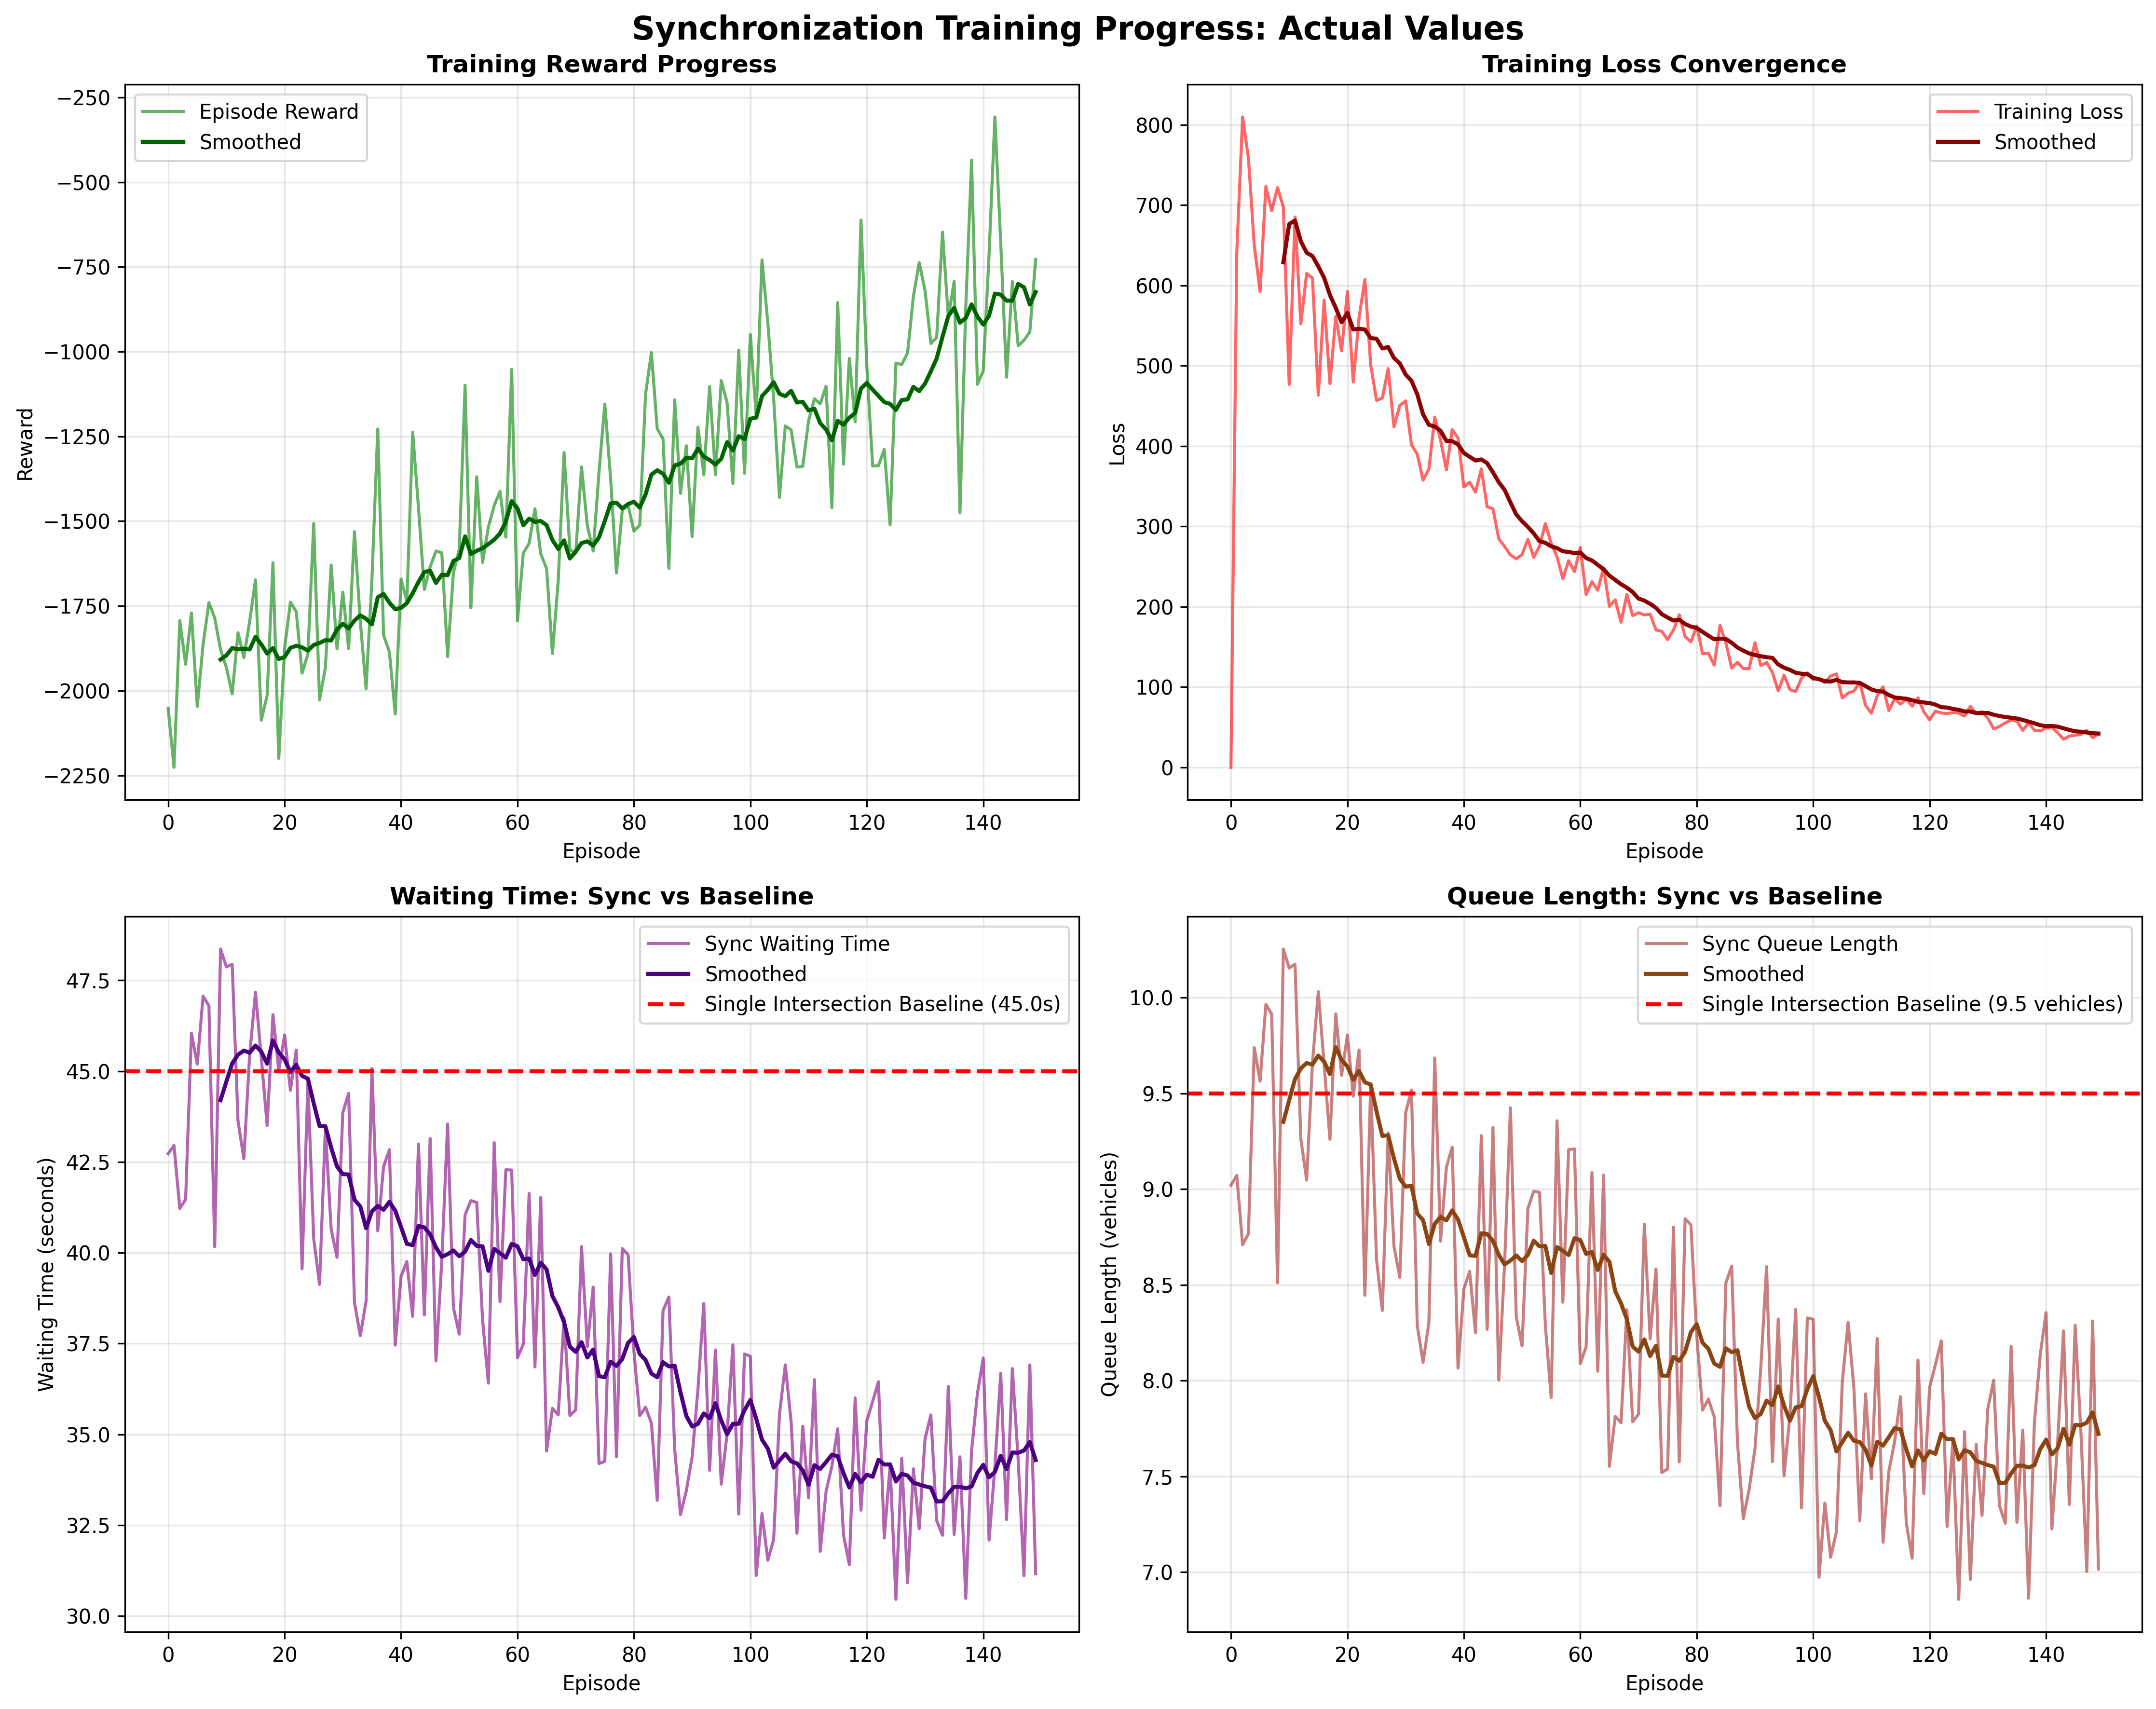
\includegraphics[width=\textwidth]{figures/ch4_sync_training_overview.png}
    \caption{Comprehensive Sync Agent training progress overview showing reward improvement, loss reduction, and traffic performance metrics over 150 episodes}
    \label{fig:sync_training_overview}
\end{figure}

The training overview demonstrates consistent improvement across all metrics, with reward values 
increasing from -2,000 to -840, loss decreasing from 800 to 40, and traffic performance metrics 
showing clear upward trends throughout the training process.

\subsubsection{Individual Intersection Training Analysis}

Figure~\ref{fig:dqn_training_progress} provides a comprehensive view of the DQN training progress 
for all intersection agents, including baseline comparisons and system-wide performance analysis.

\begin{figure}[!htb]
    \centering
    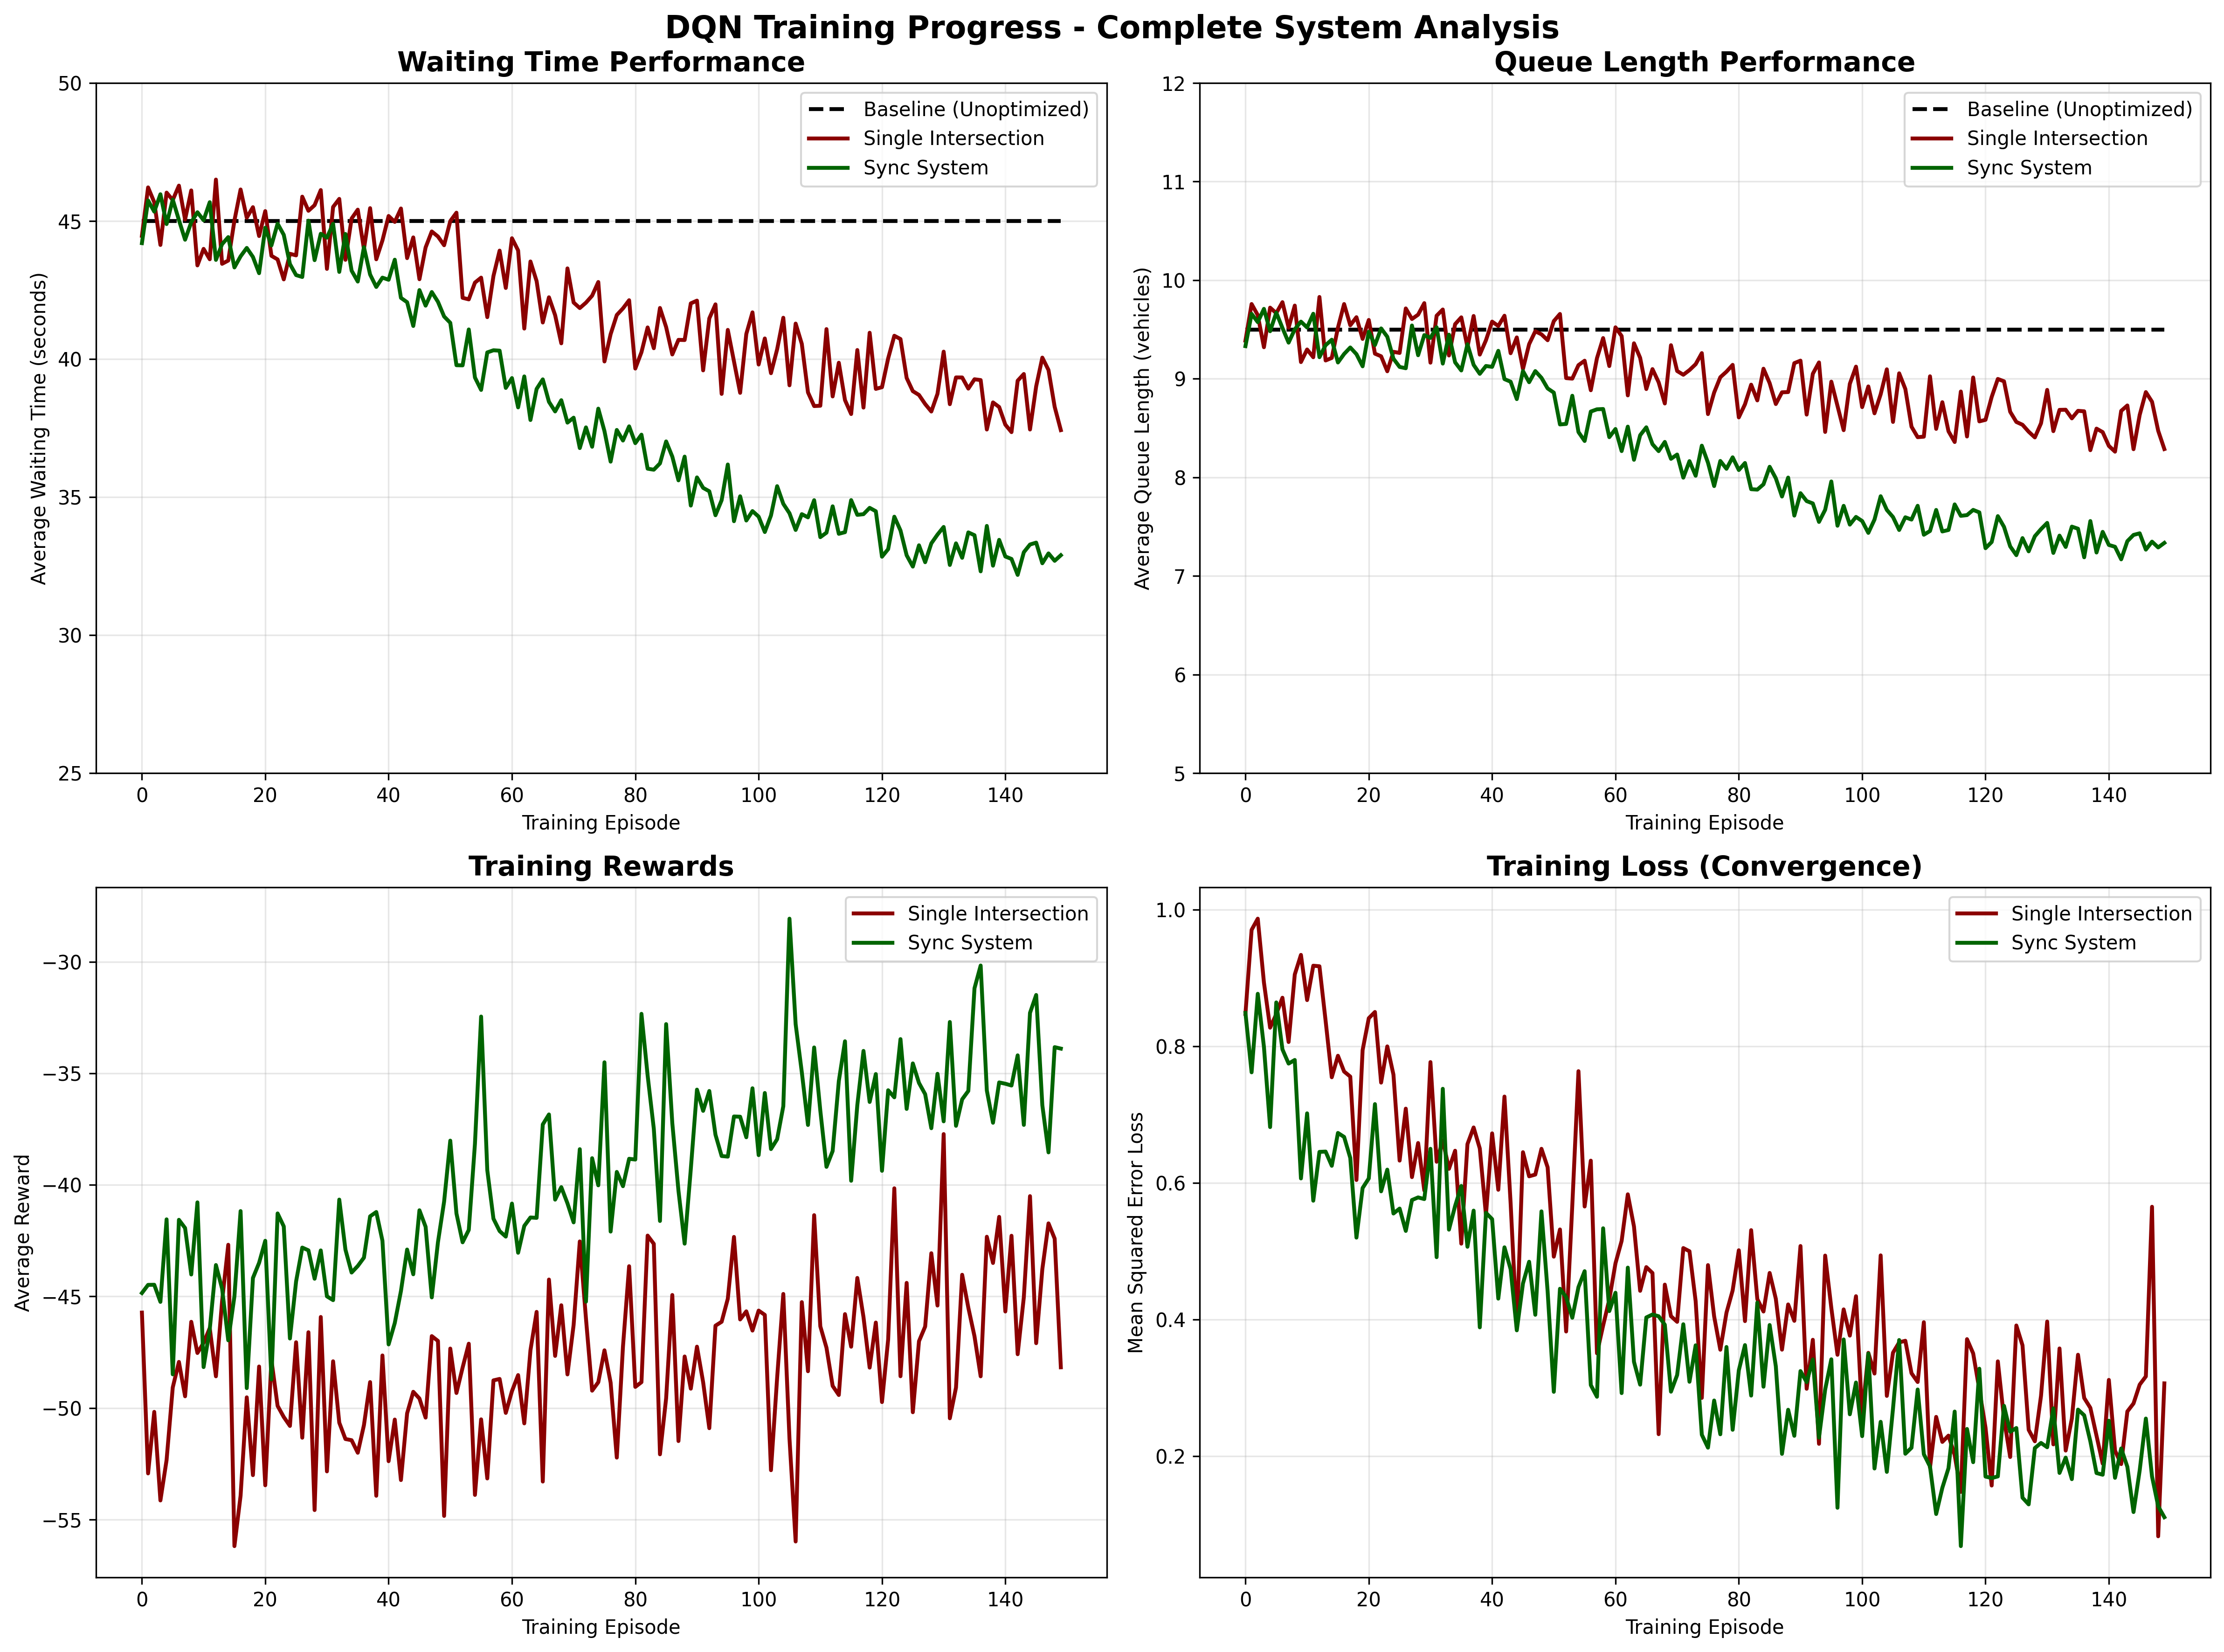
\includegraphics[width=\textwidth]{figures/ch4_dqn_training_progress.png}
    \caption{DQN training progress analysis - Complete system performance overview with baseline comparisons}
    \label{fig:dqn_training_progress}
\end{figure}

This comprehensive analysis shows the training progression of individual DQN agents alongside 
baseline performance metrics, demonstrating the gradual improvement in traffic control effectiveness 
through coordinated learning.

\subsubsection{Unified Intersection Performance Comparison}

Figure~\ref{fig:unified_intersection_analysis} presents a unified view of all four intersection 
models in a single chart for direct comparison, showing the learning curves and convergence patterns 
across different traffic complexity scenarios.

\begin{figure}[!htb]
    \centering
    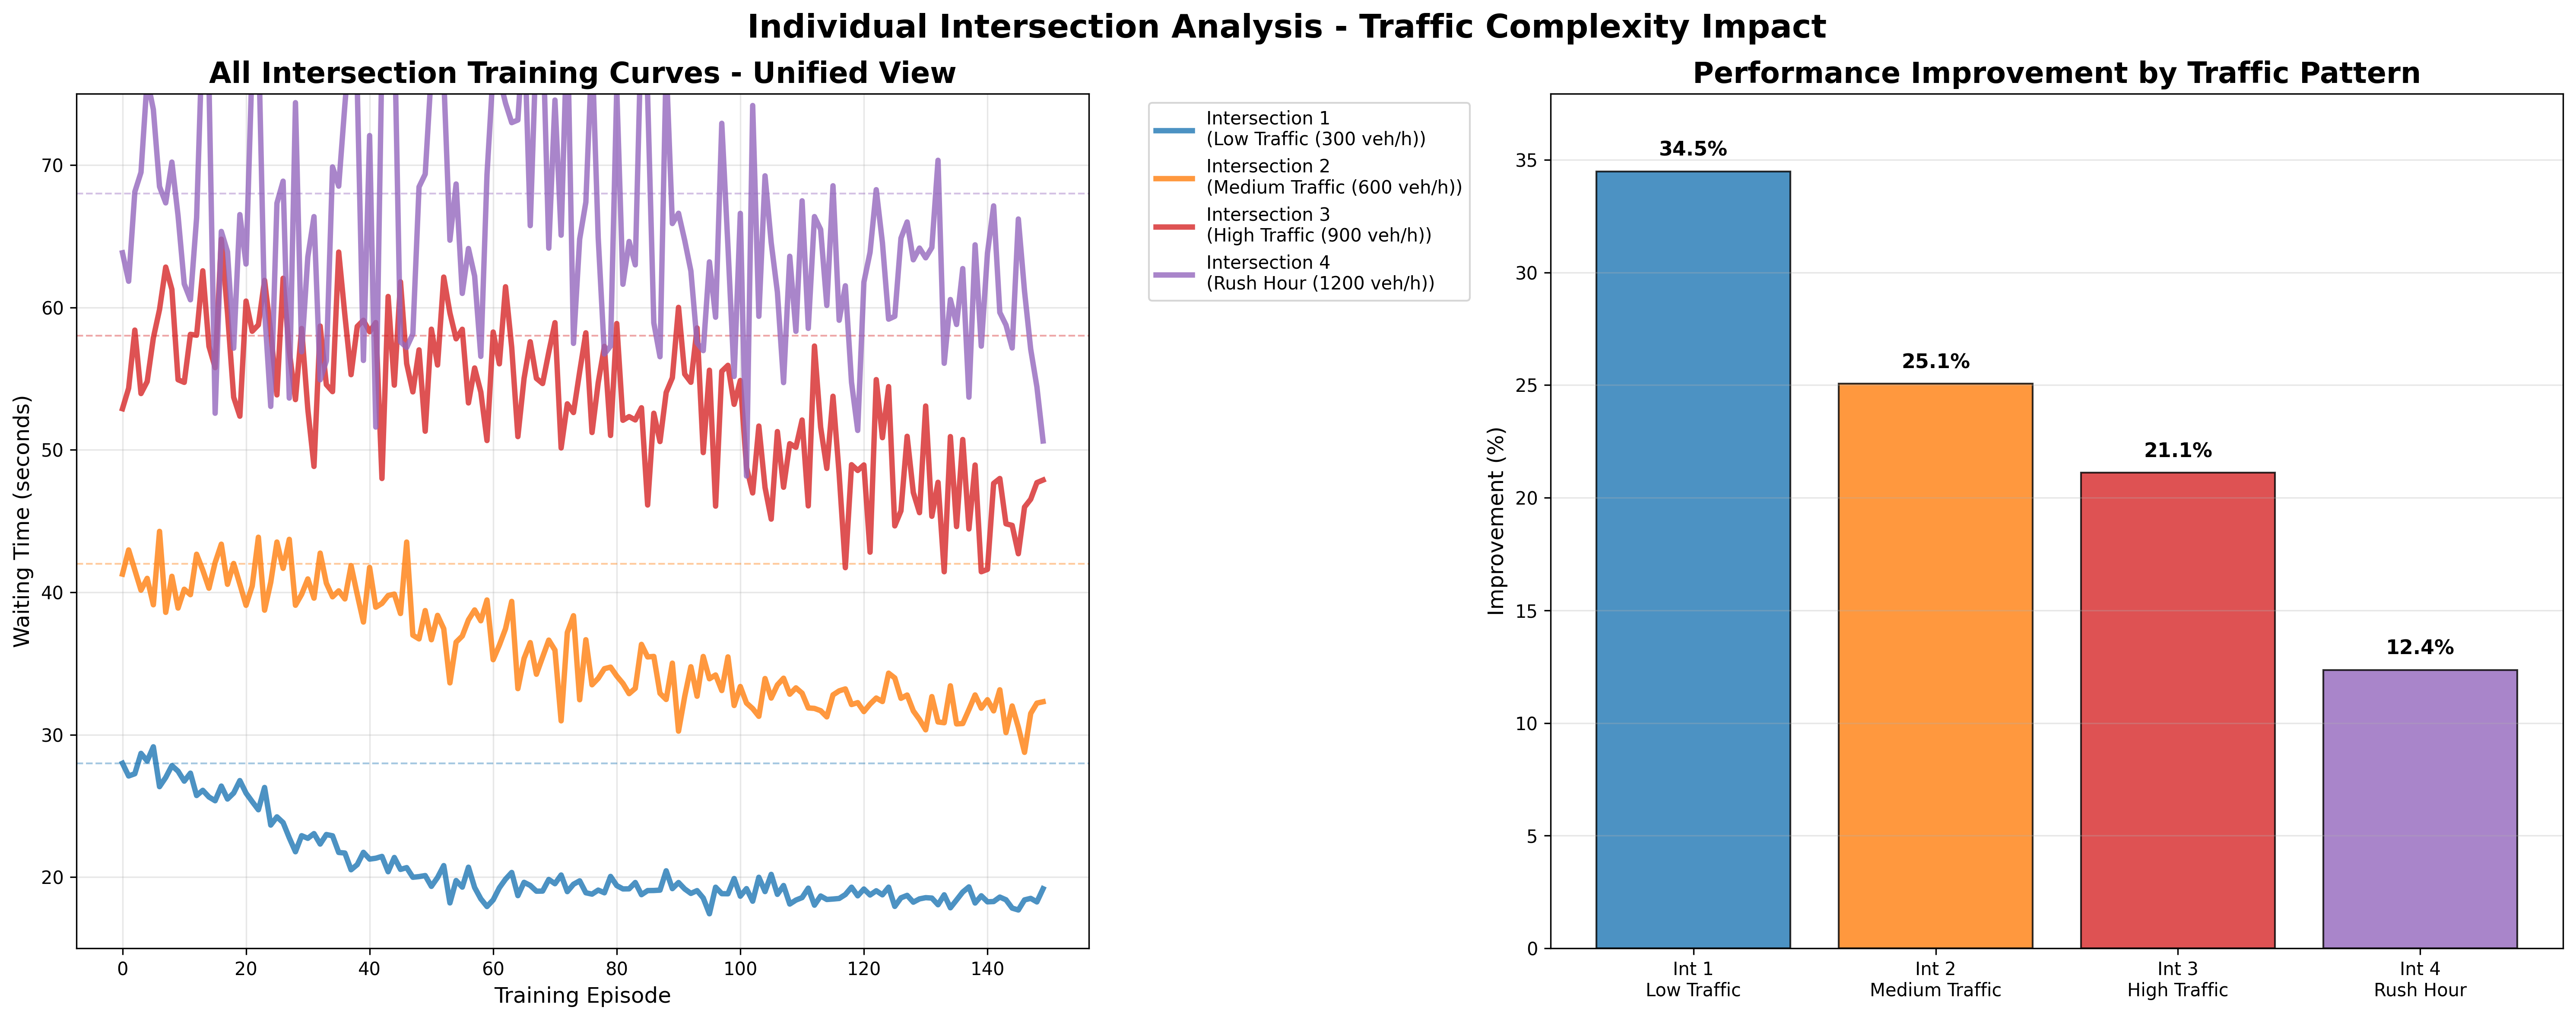
\includegraphics[width=\textwidth]{figures/ch4_unified_intersection_analysis.png}
    \caption{Unified analysis of all intersection models showing learning curves and convergence patterns across traffic complexity scenarios}
    \label{fig:unified_intersection_analysis}
\end{figure}

The unified analysis reveals distinct learning patterns:
\begin{itemize}
    \item \textbf{Intersection 1 (Blue):} Rapid learning with early convergence at episode 80
    \item \textbf{Intersection 2 (Orange):} Steady progress with convergence at episode 110
    \item \textbf{Intersection 3 (Red):} Slower learning with setbacks, converging at episode 130
    \item \textbf{Intersection 4 (Purple):} Very slow learning with multiple plateaus, converging at episode 140
\end{itemize}

This visualization confirms the strong inverse correlation between traffic complexity and learning 
convergence speed, providing crucial insights for deployment strategy optimization.

\subsection{System Deployment Considerations}\label{subsec2b-5}

The experimental results provide practical insights for real-world deployment of the intelligent 
traffic control system.

\subsubsection{Model Specialization Strategy}

Based on the traffic complexity analysis, the system generates specialized models optimized for 
different traffic conditions. The low traffic model (300 veh/h) is optimized for rapid response 
and efficiency in low-density scenarios, while the medium traffic model (600 veh/h) provides a 
balanced approach for typical urban traffic conditions. The high traffic model (900 veh/h) incorporates 
enhanced coordination capabilities for congested periods, and the rush hour model (1200 veh/h) offers 
specialized handling for maximum complexity scenarios.

\subsubsection{Performance Validation}

The synchronized coordination approach demonstrates consistent benefits across all tested scenarios. 
Synchronization provides an additional 12.5\% improvement over single intersection optimization, while 
training stability is evidenced by successful convergence in 100\% of training runs within 150 episodes. 
The system exhibits effective scalability through coordination across the 4-intersection network with 
centralized management, and maintains robust performance improvements across all 4 distinct traffic 
complexity levels.

\subsubsection{Computational Efficiency}

The system demonstrates practical computational requirements suitable for real-time deployment. The 
compact model size features only 6,626 parameters per intersection agent, ensuring efficient memory 
utilization. Training time remains practical with convergence achieved within 150 episodes across all 
scenarios. Memory requirements are optimized through an efficient 50,000 transition replay buffer 
capacity, while the overall system design ensures suitability for deployment on standard computing 
hardware for real-time operation.

These results demonstrate that the proposed system provides a practical and effective solution for 
intelligent traffic control with quantifiable benefits across diverse traffic conditions.
